\documentclass{article}

% If you're new to LaTeX, here's some short tutorials:
% https://www.overleaf.com/learn/latex/Learn_LaTeX_in_30_minutes
% https://en.wikibooks.org/wiki/LaTeX/Basics

% Formatting
\usepackage{tikz}
\usepackage{subfig}
\usepackage{hyperref}
\usepackage{subcaption}
\usepackage[utf8]{inputenc}
\usepackage[margin=1in]{geometry}
\usepackage[titletoc,title]{appendix}

% Math
% https://www.overleaf.com/learn/latex/Mathematical_expressions
% https://en.wikibooks.org/wiki/LaTeX/Mathematics
\usepackage{amsmath,amsfonts,amssymb,mathtools}

% Images
% https://www.overleaf.com/learn/latex/Inserting_Images
% https://en.wikibooks.org/wiki/LaTeX/Floats,_Figures_and_Captions
\usepackage{graphicx,float}

% Tables
% https://www.overleaf.com/learn/latex/Tables
% https://en.wikibooks.org/wiki/LaTeX/Tables

% Algorithms
% https://www.overleaf.com/learn/latex/algorithms
% https://en.wikibooks.org/wiki/LaTeX/Algorithms
\usepackage[ruled,vlined]{algorithm2e}
\usepackage{algorithmic}

% Code syntax highlighting
% https://www.overleaf.com/learn/latex/Code_Highlighting_with_minted
\usepackage{minted}
\usemintedstyle{borland}

% References
% https://www.overleaf.com/learn/latex/Bibliography_management_in_LaTeX
% https://en.wikibooks.org/wiki/LaTeX/Bibliography_Management
\usepackage{biblatex}
\addbibresource{references.bib}

% Title content
\title{
    \textbf{CSE343: Machine Learning} \\ \vspace*{-5pt}
    \textbf{\large{Assignment-4}}
}

\author{\href{mailto:shubham21099@iiitd.ac.in}{Shubham Sharma (2021099)}}
\date{\today}

\geometry{a4paper, left=20mm, right=20mm, top=20mm, bottom=20mm}

\begin{document}

\maketitle

% Abstract
% \begin{abstract}
%     Add your abstract here.
% \end{abstract}

% Introduction and Overview
\section{Section A (Theoretical)}
% Add your introduction and overview here.

% Example Subsection
\subsection*{Solution (a)}
\subsection*{(a) Dimensions of the Resulting Feature Map}
For a convolutional layer with stride \( S = 1 \) and no padding:
\[
\text{Output height} = M - K + 1
\]
\[
\text{Output width} = N - K + 1
\]
Thus, the dimensions of the resulting feature map are:
\[
(M - K + 1) \times (N - K + 1)
\]

\subsection*{(b) Number of Elementary Operations per Output Pixel}
For a single output pixel, the kernel of size \( K \times K \) is applied to the input channels.
\begin{itemize}
    \item \textbf{Multiplications:} For \( P \) channels, there are \( P \cdot K^2 \) multiplications.
    \item \textbf{Additions:} Summing the results of the \( P \cdot K^2 \) multiplications involves \( P \cdot K^2 - 1 \) additions.
\end{itemize}
\[
\text{Total operations} = P \cdot K^2 + (P \cdot K^2 - 1) = 2 \cdot P \cdot K^2 - 1 \approx 2 \cdot P \cdot K^2
\]

\subsection*{(c) Computational Time Complexity}
\begin{enumerate}
    \item \textbf{Number of Output Pixels:} For a feature map of size \((M - K + 1) \times (N - K + 1)\), the total number of output pixels is:
    \[
    (M - K + 1) \cdot (N - K + 1)
    \]
    \item \textbf{Operations for One Kernel:} For each kernel, computing the entire feature map requires:
    \[
    (M - K + 1) \cdot (N - K + 1) \cdot (2 \cdot P \cdot K^2)
    \]
    \item \textbf{Operations for \( Q \) Kernels:} With \( Q \) kernels, the total computational cost is:
    \[
    Q \cdot (M - K + 1) \cdot (N - K + 1) \cdot (2 \cdot P \cdot K^2)
    \]
    The time complexity is therefore:
    \[
    O(Q \cdot (M - K) \cdot (N - K) \cdot P \cdot K^2)
    \]
    \item \textbf{For \( \min(M, N) \gg K \):} When \( K \) is much smaller than \( \min(M, N) \). The time complexity simplifies to:
    \[
    O(Q \cdot M \cdot N \cdot P \cdot K^2)
    \]
\end{enumerate}


\vspace{10pt}
\subsection*{Solution (b)}
\subsection*{K-Means Algorithm: Assignment and Update Steps}

K-Means is an iterative clustering algorithm that partitions a dataset into $K$ clusters.

\subsubsection*{Assignment Step}
Each data point is assigned to the cluster whose centroid is closest to it. The distance is computed using the Euclidean distance formula:
\[
\text{distance} = \sqrt{\sum_{i=1}^{n} (x_i - c_i)^2}
\]
where $x$ is the data point, $c$ is the centroid, and $n$ is the dimension of the data.

\subsubsection*{Update Step}
After assigning all points to clusters, the centroids of the clusters are recalculated as the mean of all the data points assigned to that cluster:
\[
c_j = \frac{1}{n_j} \sum_{i=1}^{n_j} x_i
\]
where $c_j$ is the updated centroid of cluster $j$, $n_j$ is the number of points in cluster $j$, and $x_i$ are the points in the cluster.

\vspace{10pt}
\hspace{-15pt}Both of the above steps are repeated until convergence, i.e., when the cluster assignments no longer change or the centroid movements fall below a threshold.

\subsection*{Determining the Optimal Number of Clusters}

\subsubsection*{Elbow Method}
This method involves plotting the \textit{within-cluster sum of squares (WCSS)} for different values of $K$, where:
\[
\text{WCSS} = \sum_{j=1}^{K} \sum_{i=1}^{n_j} \|x_i - c_j\|^2
\]
Here, $\|x_i - c_j\|^2$ is the squared distance between a point and its cluster centroid.

\vspace{10pt}
\hspace{-15pt}As $K$ increases, WCSS decreases because more clusters mean that each cluster has fewer points and is more compact. The optimal $K$ is chosen at the "elbow point" in the plot, where the rate of decrease in WCSS slows significantly.

\subsection*{Random Initialization of Centroids and Global Minima}

\subsubsection*{Random Initialization}
In K-Means, initial centroids can be chosen randomly. However, the quality of the final clusters depends on the initialization of centroids. Random initialization can lead to suboptimal solutions (local minima) because the algorithm may converge to a local minimum.

\subsubsection*{Global Minima}
K-Means is not guaranteed to find the global minimum due to its sensitivity to initialization. To tackle this, there are other versions of KMeans, such as \textit{K-Means++}, which select initial centroids in a more informed manner to increase the likelihood of convergence to a global minimum.


\vspace{10pt} % add 10pt of vertical space
\section{Section B (Scratch Implementation)}
\subsection*{Part B: Final Centroids and Visualization of Clusters}
\subsubsection*{a) Final Centroids}
\[
\text{Final Centroids} = \{\textbf{(5.8, 2.125), (4.19, -0.05)}\}
\]
\subsubsection*{b) Clusters Visualization}
\begin{figure}[H] % h = here, t = top, b = bottom, etc.
    \centering
    \begin{minipage}{1\linewidth}
        \centering
        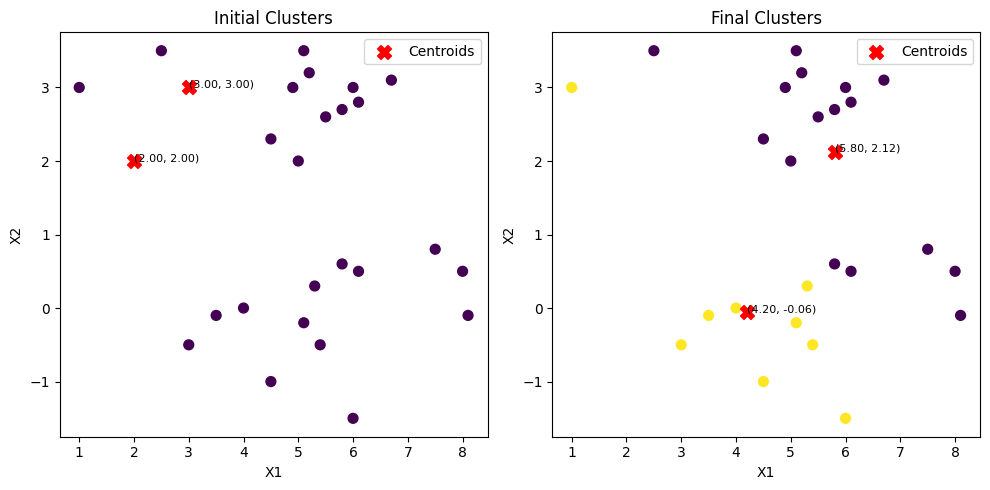
\includegraphics[scale=0.4]{assets/b.png}
        \caption{Comparision of Centroids Before and After the Algorithm Converges}{}
        \label{fig:1c}
    \end{minipage}
\end{figure}

\subsection*{Part C: Random Centroids and Visualization of Clusters}
\subsubsection*{a) Final Centroids after Random Initialization of Centroids}
\[
\text{Final Centroids} = \{\textbf{(4.85, 2.89), (5.56, -0.09)}\}
\]
\subsubsection*{b) Clusters Visualization}
\begin{figure}[H] % h = here, t = top, b = bottom, etc.
    \centering
    \begin{minipage}{1\linewidth}
        \centering
        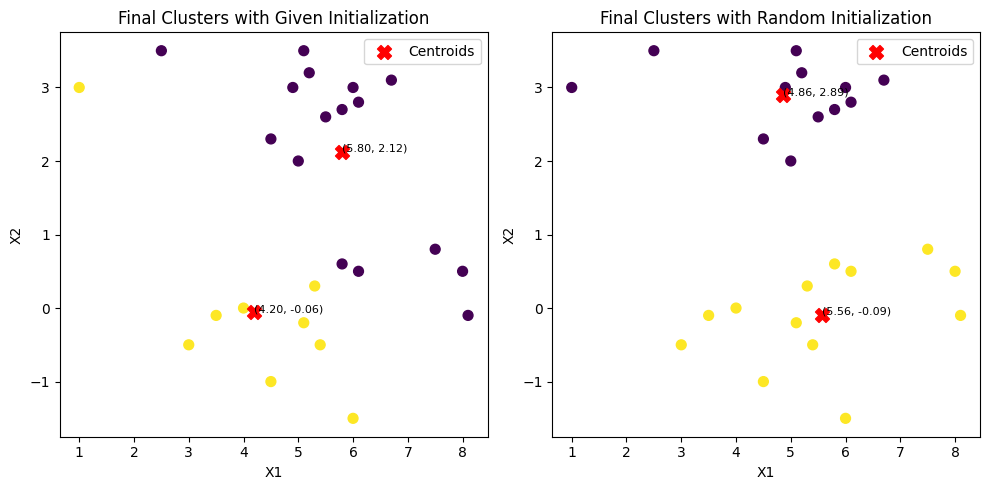
\includegraphics[scale=0.4]{assets/c.png}
        \caption{Comparision of Centroids After Given Initialization and After the Random Initialization}{}
        \label{fig:1c}
    \end{minipage}
\end{figure}

From the above graphs, I observed that the final cluster formed by randomly initialized centroids is much more compact and better than the initially given centroids.


\subsection*{Part D: Determining Optimal Number of Clusters using Elbow Method}
\begin{figure}[H] % h = here, t = top, b = bottom, etc.
    \centering
    \begin{minipage}{1\linewidth}
        \centering
        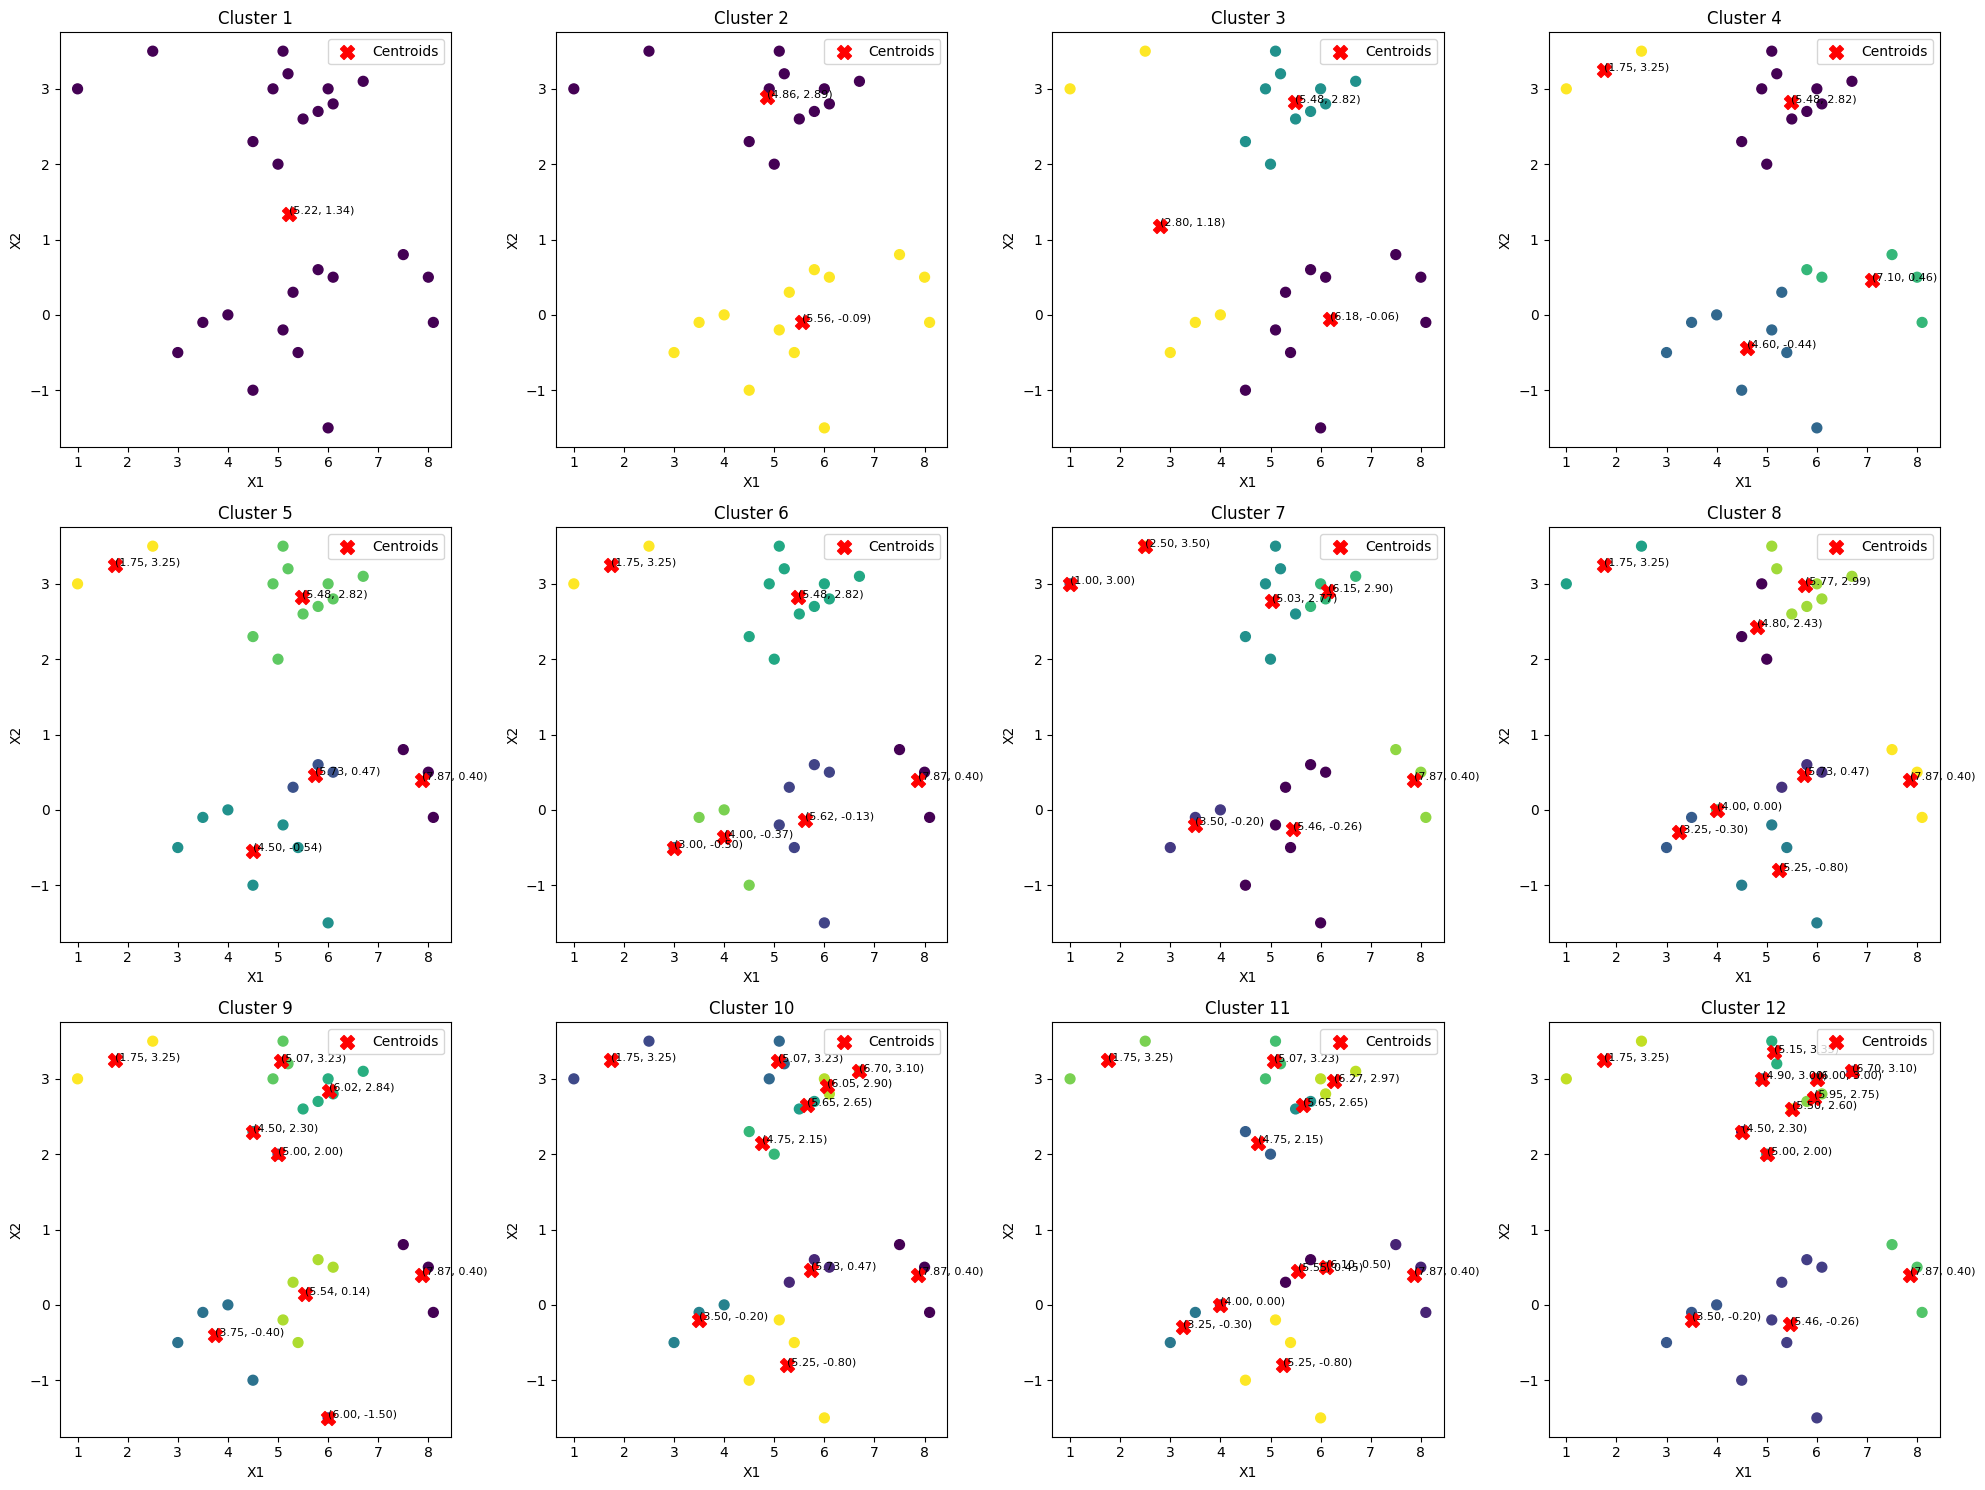
\includegraphics[scale=0.35]{assets/d-a.png}
        \caption{Final Centroids against different values of k}{}
        \label{fig:1c}
    \end{minipage}
\end{figure}

\begin{figure}[H] % h = here, t = top, b = bottom, etc.
    \centering
    \begin{minipage}{1\linewidth}
        \centering
        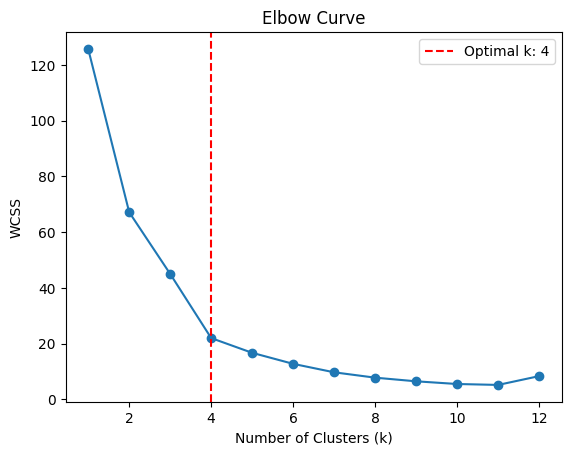
\includegraphics[scale=0.35]{assets/d-b.png}
        \caption{Within-Cluster Sum of Squares (WCSS) against different values of k}{}
        \label{fig:1c}
    \end{minipage}
\end{figure}

From the above graph, it is clearly visible that as the value of k is increasing, the WCSS score is decreasing, and the point where the rate of decrease in WCSS slows significantly is chosen as the Elbow point, and we get the optimal number of k value.
\[
\text{Optimal Value of K} = \textbf{4}
\]




% \clearpage % This ensures the page break happens here

% \vspace{10pt}
% \subsection*{Solution (f)}
% \subsubsection*{Early Stopping and its Effect of Overfitting and Generalization}
% \begin{figure}[H] % h = here, t = top, b = bottom, etc.
%     \centering
%     \begin{minipage}{0.49\linewidth}
%         \centering
%         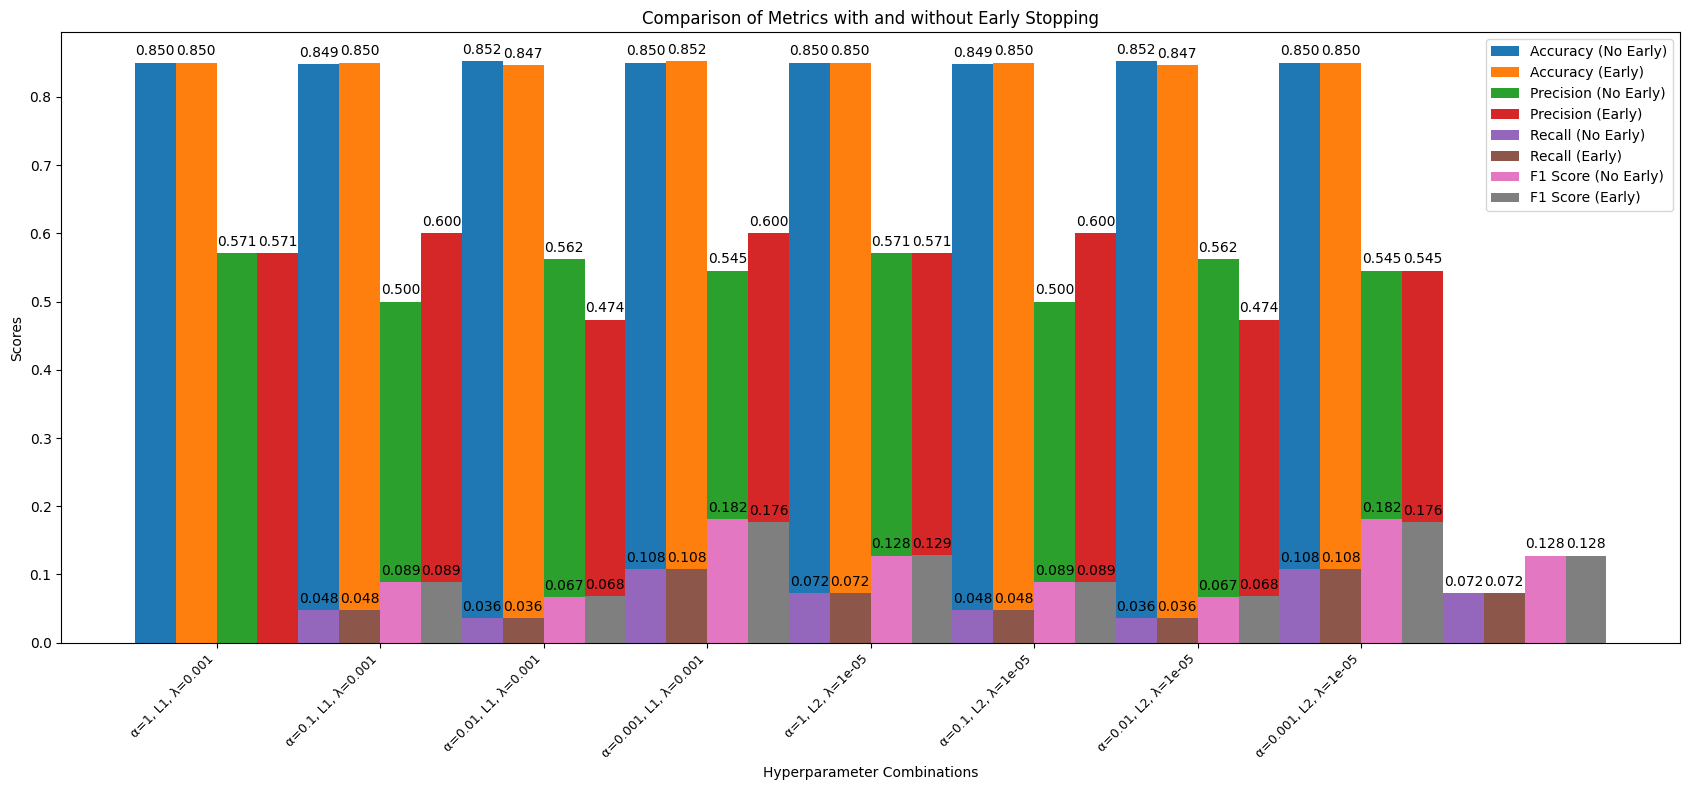
\includegraphics[width=\linewidth]{assets/fV.png}
%         \caption{Validation Dataset}{}
%         \label{fig:b-1}
%     \end{minipage}
%     \hfill
%     \begin{minipage}{0.49\linewidth}
%         \centering
%         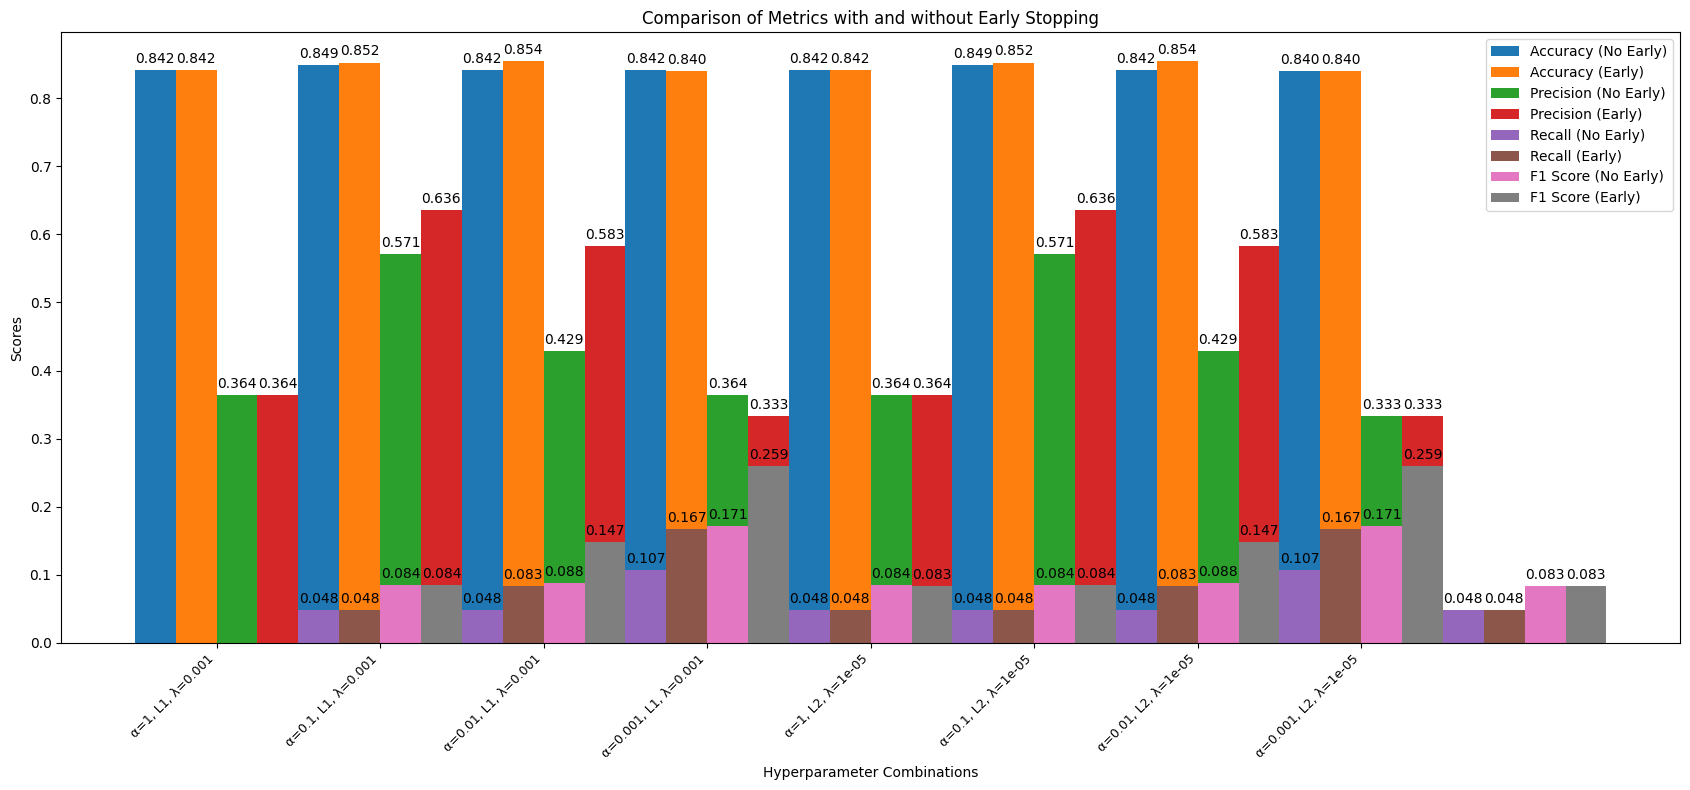
\includegraphics[width=\linewidth]{assets/fT.png}
%         \caption{Test Dataset}{}
%         \label{fig:b-2}
%     \end{minipage}
%     \caption*{Comparing impact of Early Stopping \& No Early Stopping}
% \end{figure}

% \hspace{-20pt}
% \begin{table}[H]
% \centering
% \resizebox{\textwidth}{!}{
% \begin{tabular}{|c|c|c|c|c|c|c|}
% \hline
% $\alpha$ & Regularization & $\lambda$ & Accuracy (ES/NO-ES) & Precision (ES/NO-ES) & Recall (ES/NO-ES) & F1 (ES/NO-ES) \\ 
% \hline
% 1     & L1  & 0.001  & (0.8415, 0.8415) & (0.3636, 0.3636) & (0.0476, 0.0476) & (0.0842, 0.0842) \\ \hline
% 0.1   & L1  & 0.001  & (0.8525, 0.8488) & (0.6364, 0.5714) & (0.0833, 0.0476) & (0.1474, 0.0879) \\ \hline
% 0.01  & L1  & 0.001  & (0.8543, 0.8415) & (0.5833, 0.4286) & (0.1667, 0.1071) & (0.2593, 0.1714) \\ \hline
% 0.001 & L1  & 0.001  & (0.8397, 0.8415) & (0.3333, 0.3636) & (0.0476, 0.0476) & (0.0833, 0.0842) \\ \hline
% 1     & L2  & 1e-05  & (0.8415, 0.8415) & (0.3636, 0.3636) & (0.0476, 0.0476) & (0.0842, 0.0842) \\ \hline
% 0.1   & L2  & 1e-05  & (0.8525, 0.8488) & (0.6364, 0.5714) & (0.0833, 0.0476) & (0.1474, 0.0879) \\ \hline
% 0.01  & L2  & 1e-05  & (0.8543, 0.8415) & (0.5833, 0.4286) & (0.1667, 0.1071) & (0.2593, 0.1714) \\ \hline
% 0.001 & L2  & 1e-05  & (0.8397, 0.8397) & (0.3333, 0.3333) & (0.0476, 0.0476) & (0.0833, 0.0833) \\ 
% \hline
% \end{tabular}
% }
% \caption{Comparison of Early Stopping (ES) and No Early Stopping (NO-ES).}
% \end{table}



% \hspace{-15pt}To prevent overfitting, I choose the early stopping parameter as patience = 10 and min\_delta = 1e-3. This means that training will stop if the validation loss does not improve by at least 1e-3 for 10 consecutive epochs.
% \vspace{5pt}
% \newline\hspace{-15pt}After trying eight different combinations of learning rate ($\alpha$) = \{1, 0.1, 0.01, 0.001\} and L1, L2 regularization, I come to the conclusion that early stopping stops the overfitting and promotes the generalization of the unseen test data. As it will be clearly visible in the metrics data. From all combinations of models in which early stopping is enabled, has better accuracy, precision, recall, and F1-score.

\end{document}
